% !TEX TS-program = pdflatex
% !TEX encoding = UTF-8 Unicode

% This is a simple template for a LaTeX document using the "article" class.
% See "book", "report", "letter" for other types of document.

\title{Understanding fetching performance on a core-fusion enabled processor}
\section{Introduction}
I want to discuss what affects overall performance in a core-fusion based on how cores fetch blocks in a core-fusion.
I'll start by describing how fetching works on core-fusion when there's only a single segment, this will be followed by how this is expanded on when we enable 4 segments per core.
Next I'll cover 2 different processors that also use core-fusion; Ipek et al.'s original Core-Fusion processor and Pricopi et al.'s Baharupi.
Once the background is all covered I'll demonstrate how different instruction block parameters will influence the overall performance of a core composition.
This involves discussing block size in terms of bytes, instructions and cycle lengths.
We'll also see how the number of segments will require different types of blocks to be maximize performance.
With all this information at hand we then pose the question of how scheduling blocks in a different order may improve performane (getting lower cycle counts), but also may help alleviate  branch prediction requirements.

\section{Setup}
In this article we assume a 16 core processor with either 1 or 4 segments per core.
A segment represents the number of blocks a core can fetch and execute in parallel, which, in EDGE will be: $128/NumberOfSegments$.
The information in the rest of the article is based on the simulator implementation, some of this can be potentially changed, but for now we're focussing on what's implemented.
To facilitate the explanations I assume a perfect instruction cache.

\section{Understanding the fetching procedure}
The fetch procedure can be broken up into 4 steps.

\begin{itemize}
\item Step 1: Fetch block header and decode it. This will give us block size, number of instructions and the address needed to make prediction.
\item Step 2: Make ICache fetch requests to fetch block.
\item Step 3: Make branch prediction.
\item Step 4: Once the branch prediction is done, see if we can make a request for a new block.
\end{itemize}

In the simulator, steps 2, 3 and 4 can potentially be done in the same cycle. We need at least 1 cycle to fetch and decode the header, and step 4 has to be done at least 1 cycle after the prediction.

\textbf{SIMULATOR NOTE}: In the simulator, there is a current condition that states that a new block can only be fetched once a previous block has finished fetching. We will discuss later on in the report how this affects performance.
The original E2 paper does not specify that blocks will be fetched in parallel and a comment in the code claims that they don't track segment fetches in parallel (hence the waiting condition).

\subsection{Fetching on a core composition}.

When cores are fused, this changes the fetching mechanics slightly.
To simplify the explanation I will redefine every step, this time when cores are fused.


\begin{itemize}
\item Step 1: Fetch block header and decode it. This will give us block size, number of instructions and the address needed to make prediction.
\item Step 2: Make ICache fetch requests to fetch block.
\item Step 3: Make branch prediction.
\item Step 4: Once the branch prediction is done, see if we can make a request for a new block.
\item Step 5: If we cannot fit the newly predicted block on our core, send a fetch request in the composition.
\end{itemize}

There is only one new step in the composition version, however, in the current setup we will see a new restriction.
The new restriction is: If you do not hold the youngest block in one of your segments then you may no longer make fetch requests.
This means that cores in a composition are not fully autonomous, they will have to wait for another core in the composition to send them a fetch signal before being able to fetch blocks.
We will see later on how that affects performance.

\section{Related architectures}

\subsection{Core-Fusion, Ipek et. al}

Core-Fusion has a Fetch Management Unit (FMU) that allows it to dispatch instructions to cores in a composition.
An FMU will receive information from a core and resends relevent fetch information to other cores in the composition.
Usually the latency from 1 core to another via the FMU is 2 cycles.

In Core-Fusion, the cores independently fetch instructions from their Icache. They can fetch, at best, 2 instructions per cycle and have a max capacitiy of 8 instructions.
The cores in a fusion will be dependent on Core-Zero for fetch alignment.
When a fetch-stall occurs, such as an i-cache miss or i-tlb miss, all cores must stall to ensure correct alignment.
Each core can conduct a single prediction per cycle, it will send those predictions/mispredictions to the FMU which selects the correct PC to inform all cores about where to fetch.
A mispeculation will cause flushing of all cores, naturally.

In their situation, the overhead of fetching is supposedly negligeable, for example on an 8 Core system it's only 3\% on SPECINT/SPECFP.
However most of their time is spent in pipeline stalls, which most likely isn't alieviated by the fact that, at best, each core can only have 8 instructions running at any point.

\subsection{Baharupi, Pricopi et. al}
This is similar to EDGE but it doesn't use the block structure.
Instead, there's a "Sentinel Instruction" which acts like a block header, informing the core on whether or not the basic block ends with a branch/fallthrough.
When a core fetches a sentinel instruction it will execute a branch and submit it to the next core in the composition.
So this is similar to EDGE with single segment.
It's slightly less efficient due to the fact that the cores do live register renaming and depend on a shared General Program Counter (GPC).
Cores can't submit blocks in parallel, instead they need to lock in the GPC when they hit a sentinel instruction.
The GPC will be locked until register renaming is finished and the branch prediction is done.
This adds an extra latency as cores will simply have to wait for these procedures to be done to get ahold of the GPC.

\subsection{Conclusion}
Most core-fusion models operate in a similar manner, that is to say cores communicate with each other via some form of branch prediction / fetch manager to determine which instructions to fetch.
Baharupi introduces a lock on a General Program Counter which can cause extra latency due to cores needing to get the lock.
Core-Fusion claims to have a very small overhead, but this is also due to the fact that each core is only ever fetching a maximum of 2 instructions per cycle.
Given that they worked with an 8 core system that means they have a maximum of 64 instructions in flight at any point.
Since cores don't require a new branch prediction to fetch instructions, this can considerably reduce the overhead of the fetching model.
This is nothing compared to what EDGE can potentially do; on an 8 Core fusion we could have 1024 instructions being fetched, which could be a result of 8 to 32 fetch requests.

Ultimately EDGE requires branch predictions like Baharupi but doesn't suffer from lock-acquiring stalls.
However, unlike Core-Fusion, we cannot simply fetch instructions in parallel as we require to have decoded headers and made predictions as to what the next block will be, which increases the latency when we have more segments and cores.

\section{On Performance}
\subsection{Motivating example}
To start things off, I want to motivate how crucial a good fetching policy is, and how the current policies regarding fetching in a core composition can penalise performance.
In this subsection I am executing a twolf\_1 microbenchmark, which involves a loop with a set of very small blocks. 
This ensures that for the most part, each core can fetch 4 blocks.
To understand how the current fetching policy affects composition performance I track specific events that happen in the processor.
These events are:
\begin{itemize}
\item The first cycle that we fetch a new block \textbf{Fetch}.
\item The cycle at which we make a prediction for the next block \textbf{Predict}.
\item The cycle at which we make an attempt to allocate a new block \textbf{Attempt}.
\item The cycle at which a core makes a fetch request to  another core \textbf{FetchReq}.
\item The cycle at which we have to flush blocks \textbf{Flush}.
\item Cycle in which the core has no blocks and is waiting \textbf{Wait}.
\end{itemize}
Figure~\ref{fig:16step} represents a slice of the twolf\_1 execution on a 16 core, 4 segment processor.
The X axis represents the cycle count and the Y axis represents a core in the composition.
Each facet represents one of the previously mentioned events, and thus, a dot represents when one of the cores in the composition logged an event, and which cycle that happened on.

The important aspects to notice are: how the fetch requests form a stair shape, which shows how long it takes for every core to be full.
This stair shape is, of course, caused by the serialisation of the block fetches and the fact that a core only starts fetching blocks once the previous core has made a request.
The second crucial bit of information is noticing how dense the Wait facet is.
As we can see, cores spend far more time waiting than they do actualy executing code.
This is due to the fact that once they have committed their blocks, they won't be provided new blocks until its parent core submits a request.
Also, looking at when cores \textbf{do} execute code, we can see that this is barely done in parallel. 
This means that the improvements expected of core-fusion are not present in this example, as the work is serialised.


Figure~\ref{fig:16step1} represents a similar slice of the twolf\_1 microbenchmark, except this time we have 16 cores fused with a single segment.
We can ignore the CacheHit event as this is not relevant in this section.
As we can see, when each core only has a single segment, it takes less time for the composition to fill up with blocks, and thus, when looking at the Wait facet, more code is being executed in parallel.
Naturally, this is due to the fact that in a single segment processor, we can only have 16 blocks in flight, compared to the 4 segment's 64, thus the overhead of fetching is reduced.
Whilst this facilitates the motivation of core fusion, having a single segment core is a waste of resources as often times the compiler will never generate blocks of 96 instructions or more.

\begin{figure}
\center
  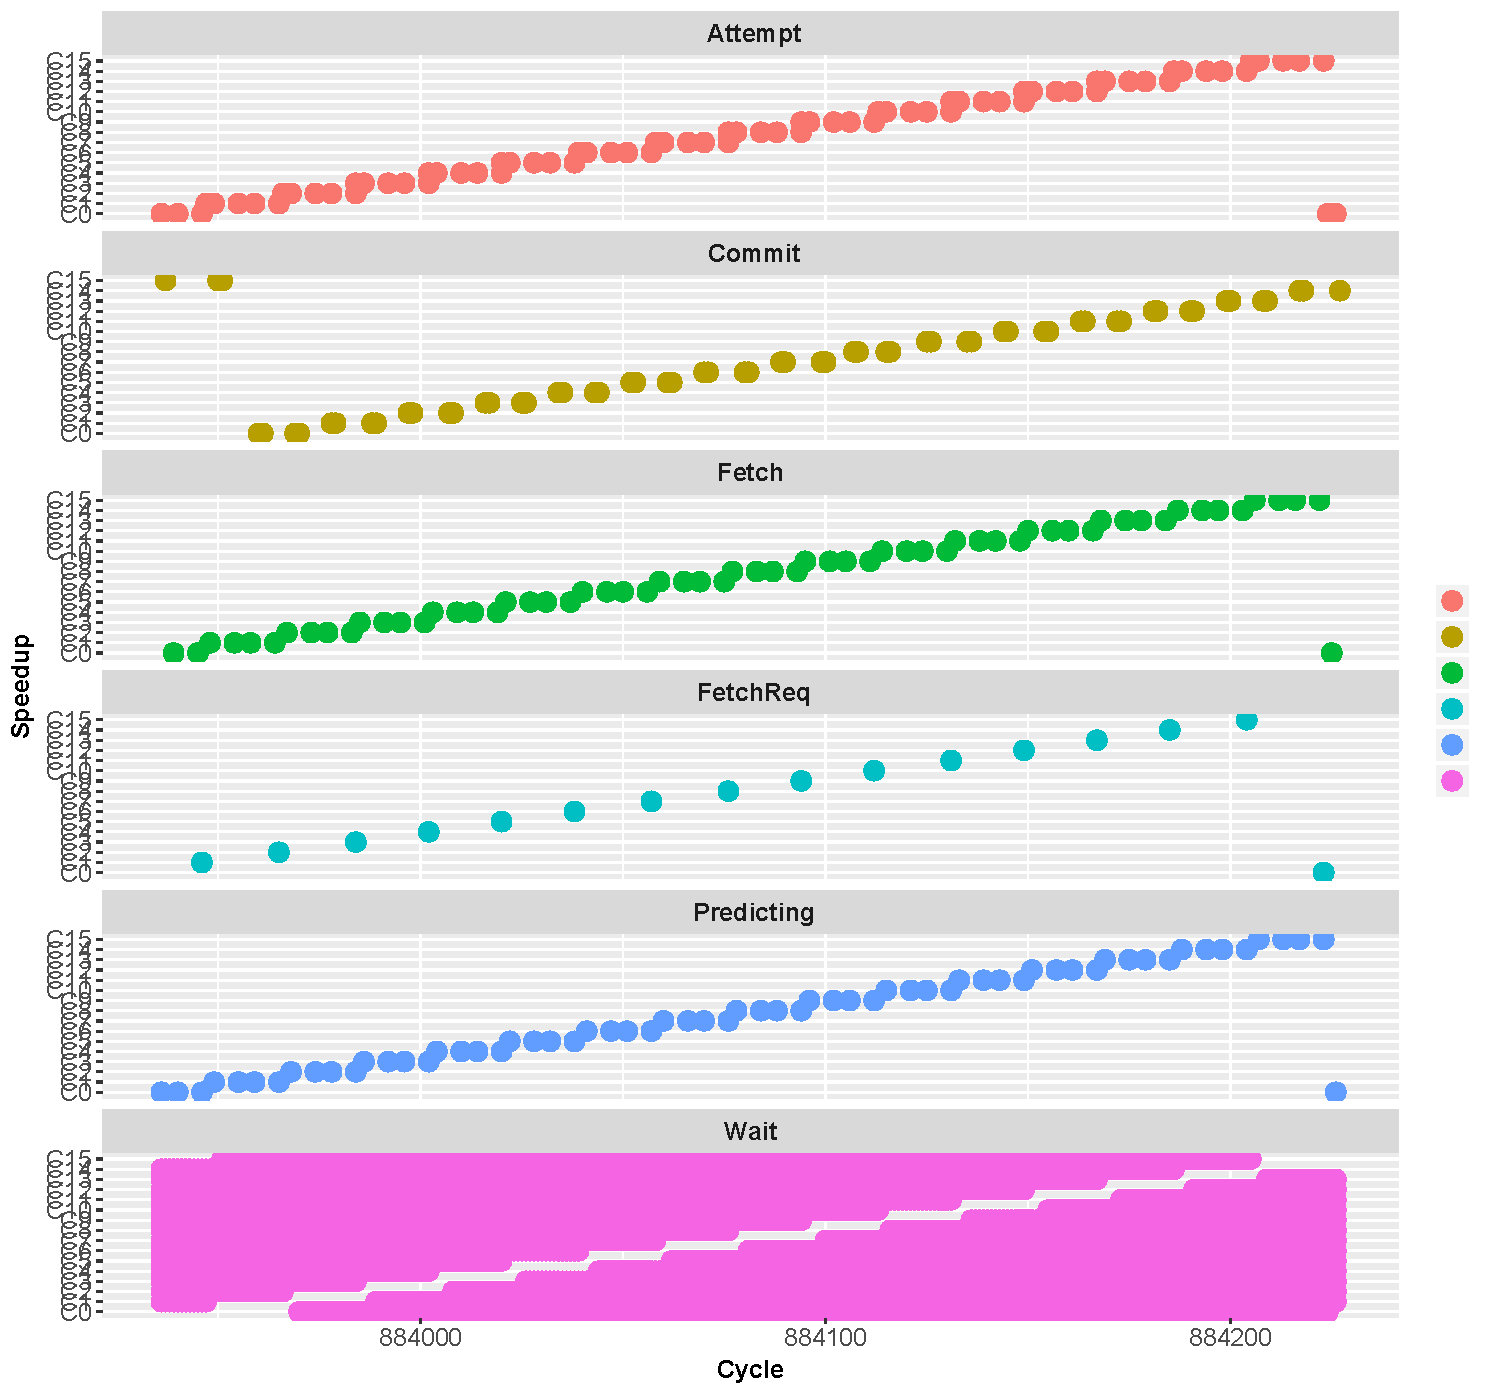
\includegraphics[width=1\textwidth]{chapter3/graphics/twolf_16.pdf}
  \caption{TWOLF on 16 cores fused, 4 segments each}\label{fig:16step}
\end{figure}

\begin{figure}
\center
  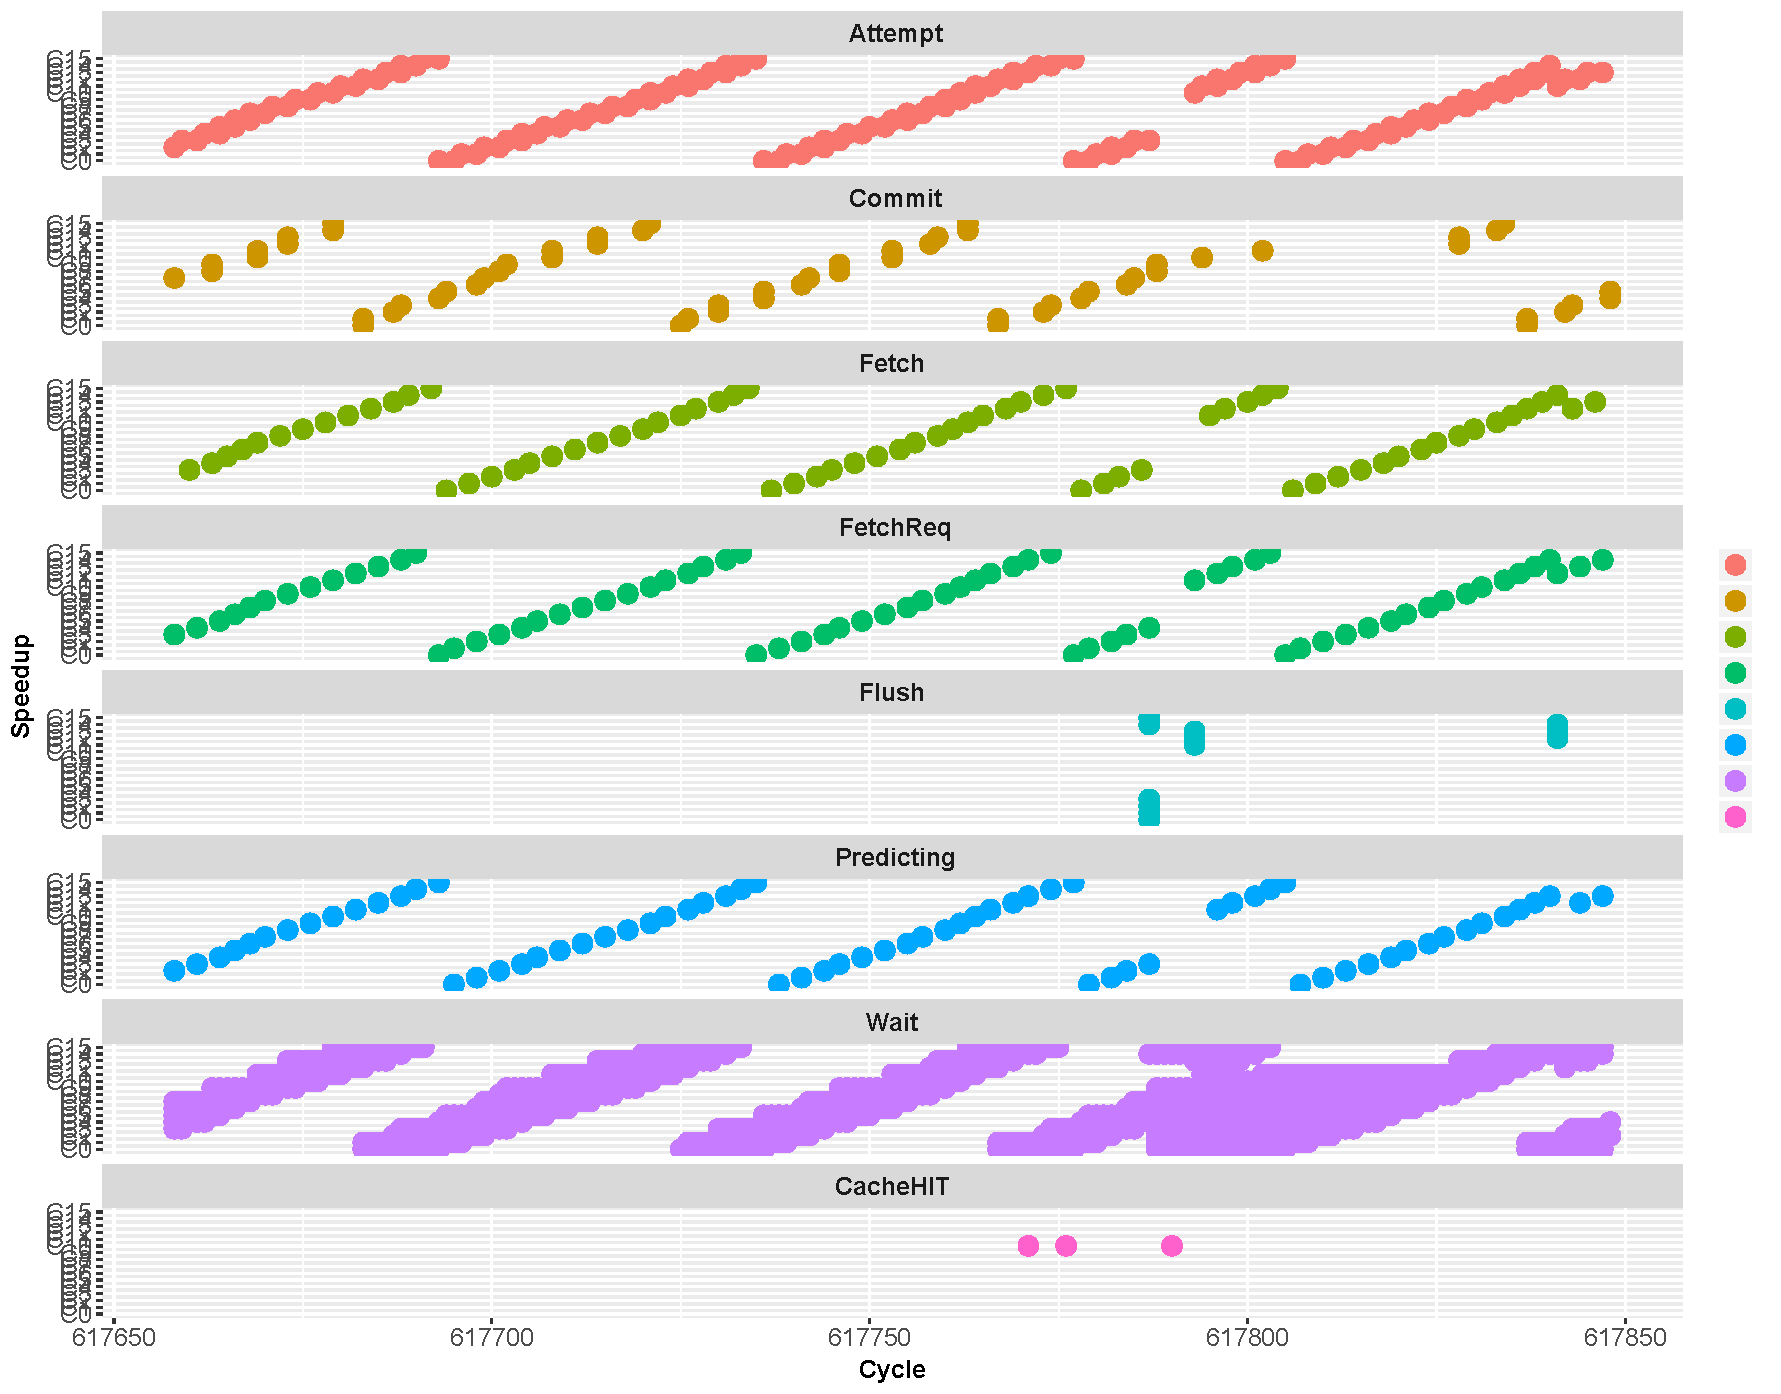
\includegraphics[width=1\textwidth]{chapter3/graphics/twolf_16_1.pdf}
  \caption{TWOLF on 16 cores fused, 1 segments each}\label{fig:16step1}
\end{figure}
\newpage
\subsection{Using synthetic benchmarks}
In the CASES paper I provided a small model to try and understand when a composition could be fully utilised in terms of IPC through the study of instructions per block.
Here we will do a study based on the actual cycle counts from different synthetic benchmarks.

\subsection{Comparing segment performance based on small blocks}
In this section I want to demonstrate how the average time it takes to execute a block in cycles affects potential speedup based on the number of segments and number of cores fused. 
In this scenario, I run a simulation where I define a block with a single instruction and manually assign the execution time of that instruction.
The blocks are independent, allowing for cores in a composition to execute in parallel.
I ran a set of experiments where I modified the number of segments, 1 or 4, number of cores fused (1,2,4,8,16) and the execution time of the block of the block (10,20,40,80,160,320 cycles).
Figure~\ref{fig:lss} represents the speedup obtained via core-fusion fusion relative to their segment count (so comparing cycle count of 1 core 1 segment with 16 core 1 segment for example).

As we can see, for a core fusion of 16 cores with 1 segment to get a 16x speedup we need independent blocks of at least 40 cycles in length.
By logging fetch requests for each core, I've noticed it takes 39 cycles for 16 cores to have a block to execute (in this example).
This is due to the fact that it takes 2 cycles to fetch header, make prediction, and send a request to another core + some extra cycles to fully fetch the block.
Since each block takes 40 cycles, this means that by the time Core 1 will have finished executing its block, Core 16 will have fetched its block and submitted a prediction and therefore Core 1 can immediately fetch a new block.
This is an ideal situation as cores are therefore always executing blocks, leading to a full utilisation.

On 4 segment cores, the picture is much less appealing; it requires blocks to take at least 160 cycles to get a 14x speedup compared to 1 Core with 4 segments.
By doing the same kind of logging as I did before, I see that with four segments, we take about 180 cycles to fill up all cores, so that means each block would at least have to be 180 cycles to be fully useful. 
Whilst this may come to no surprise, it shows that we need blocks to be at least 4x longer on a 4 segment machine compared to single segment.

So what's the point of 4 segment cores then ? It's easier to demonstrate the usefulness of core-fusion on single segment processors than it is on 4 segments.
This may be correct, but as we can see in Figure~\ref{fig:ts} where I compare the cycle counts of all executions to 1 Core 1 Segment; having 4 segments can be very beneficial.
Indeed, on longer blocks, (160 and beyond) we could, in theory, be getting up to a 64x speedup with 16 cores and a 4x speedup with just one core!
Naturally this test is synthetic, but there coudl be cases where this happens.
Having more segments not only should allow us to accomodate for smaller blocks, but also enables us to ensure that the cores can issue instructions at a more steady rate, as they can look for any available instruction from 4 blocks instead of a single 1.
Ironically this also shows that larger isn't always better, if we could generate 4 blocks that are perfectly independent and populate 16 cores with those blocks, we would technically get a better speedup than if we had 1 large block!

\begin{figure}
\center
  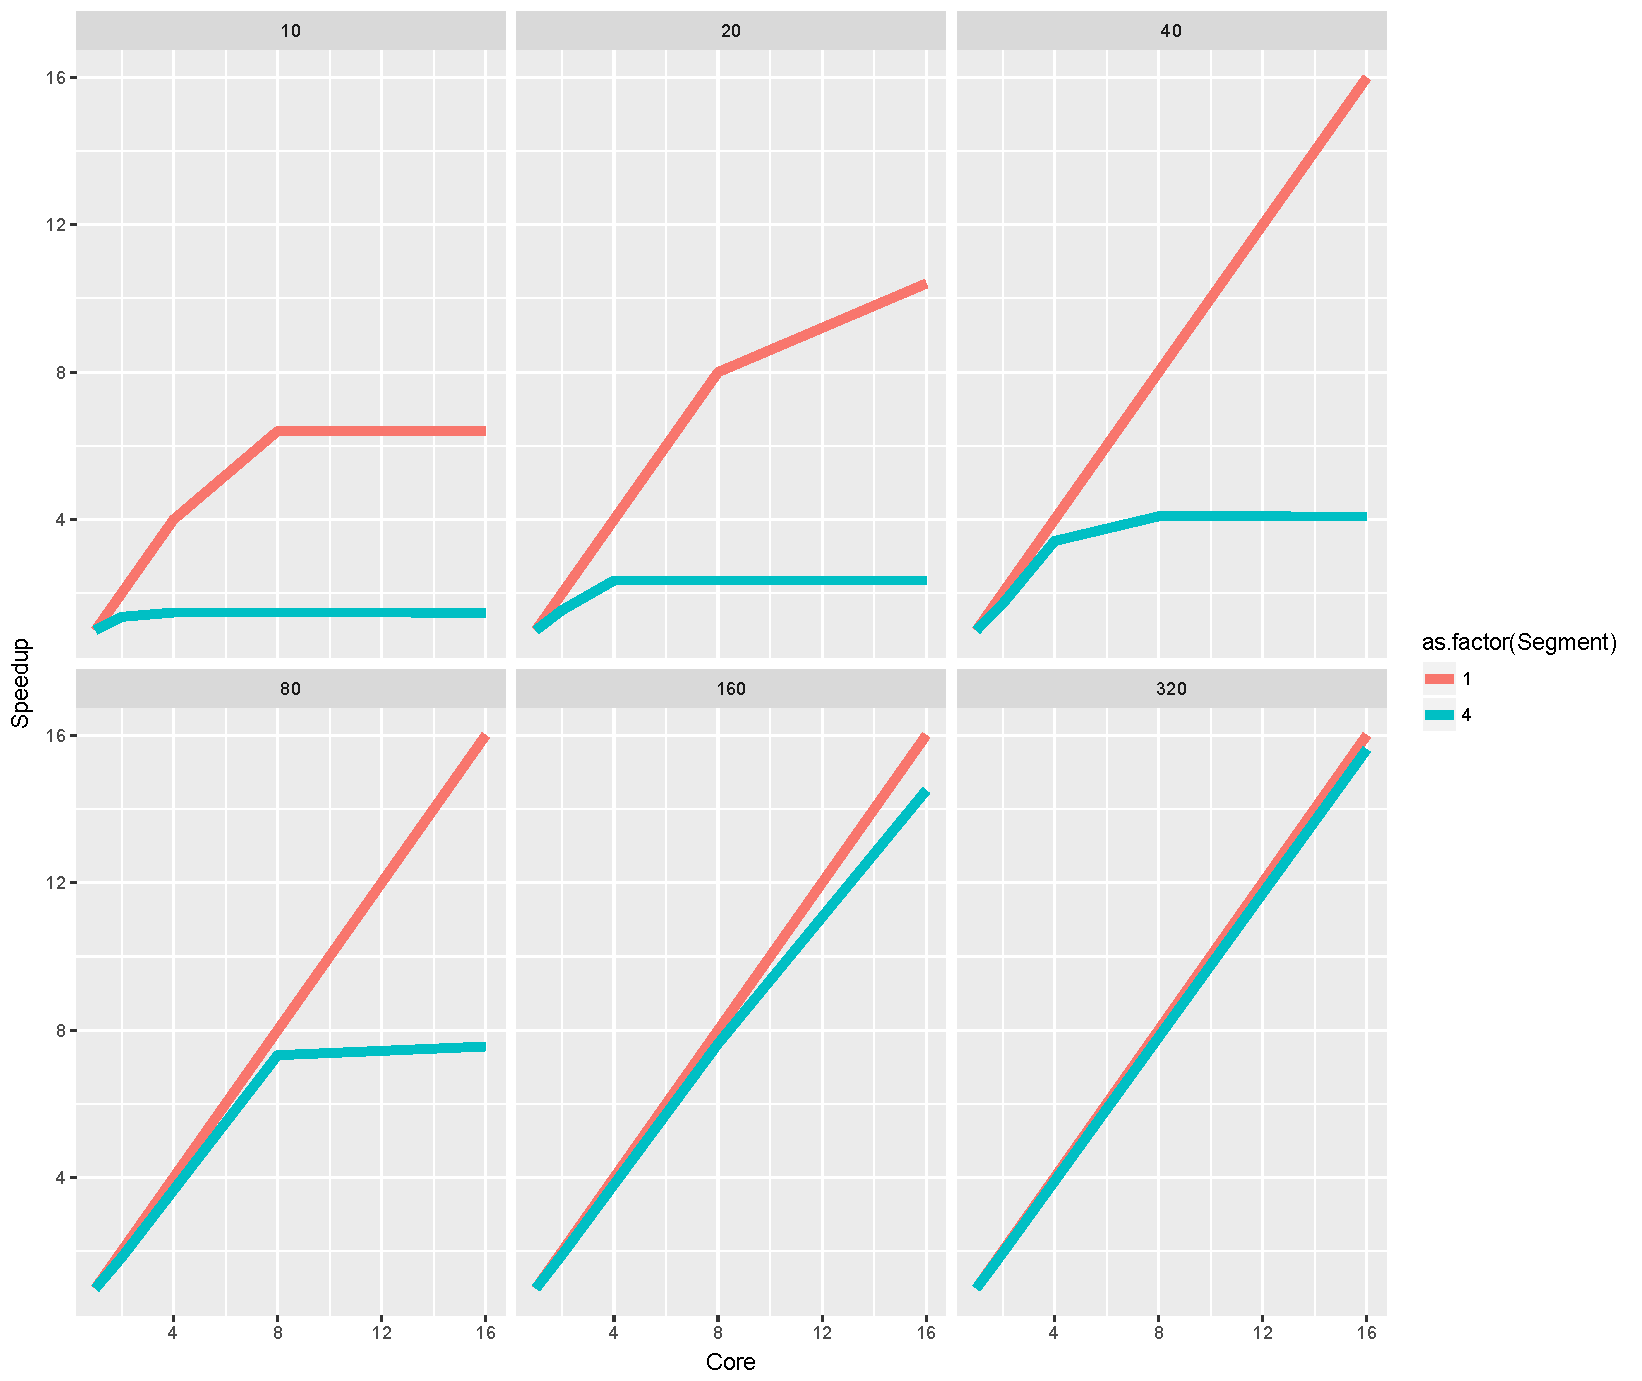
\includegraphics[width=1\textwidth]{chapter3/graphics/lengths_segment_speed.pdf}
  \caption{Speedup by segments.}\label{fig:lss}
\end{figure}

\begin{figure}
\center
  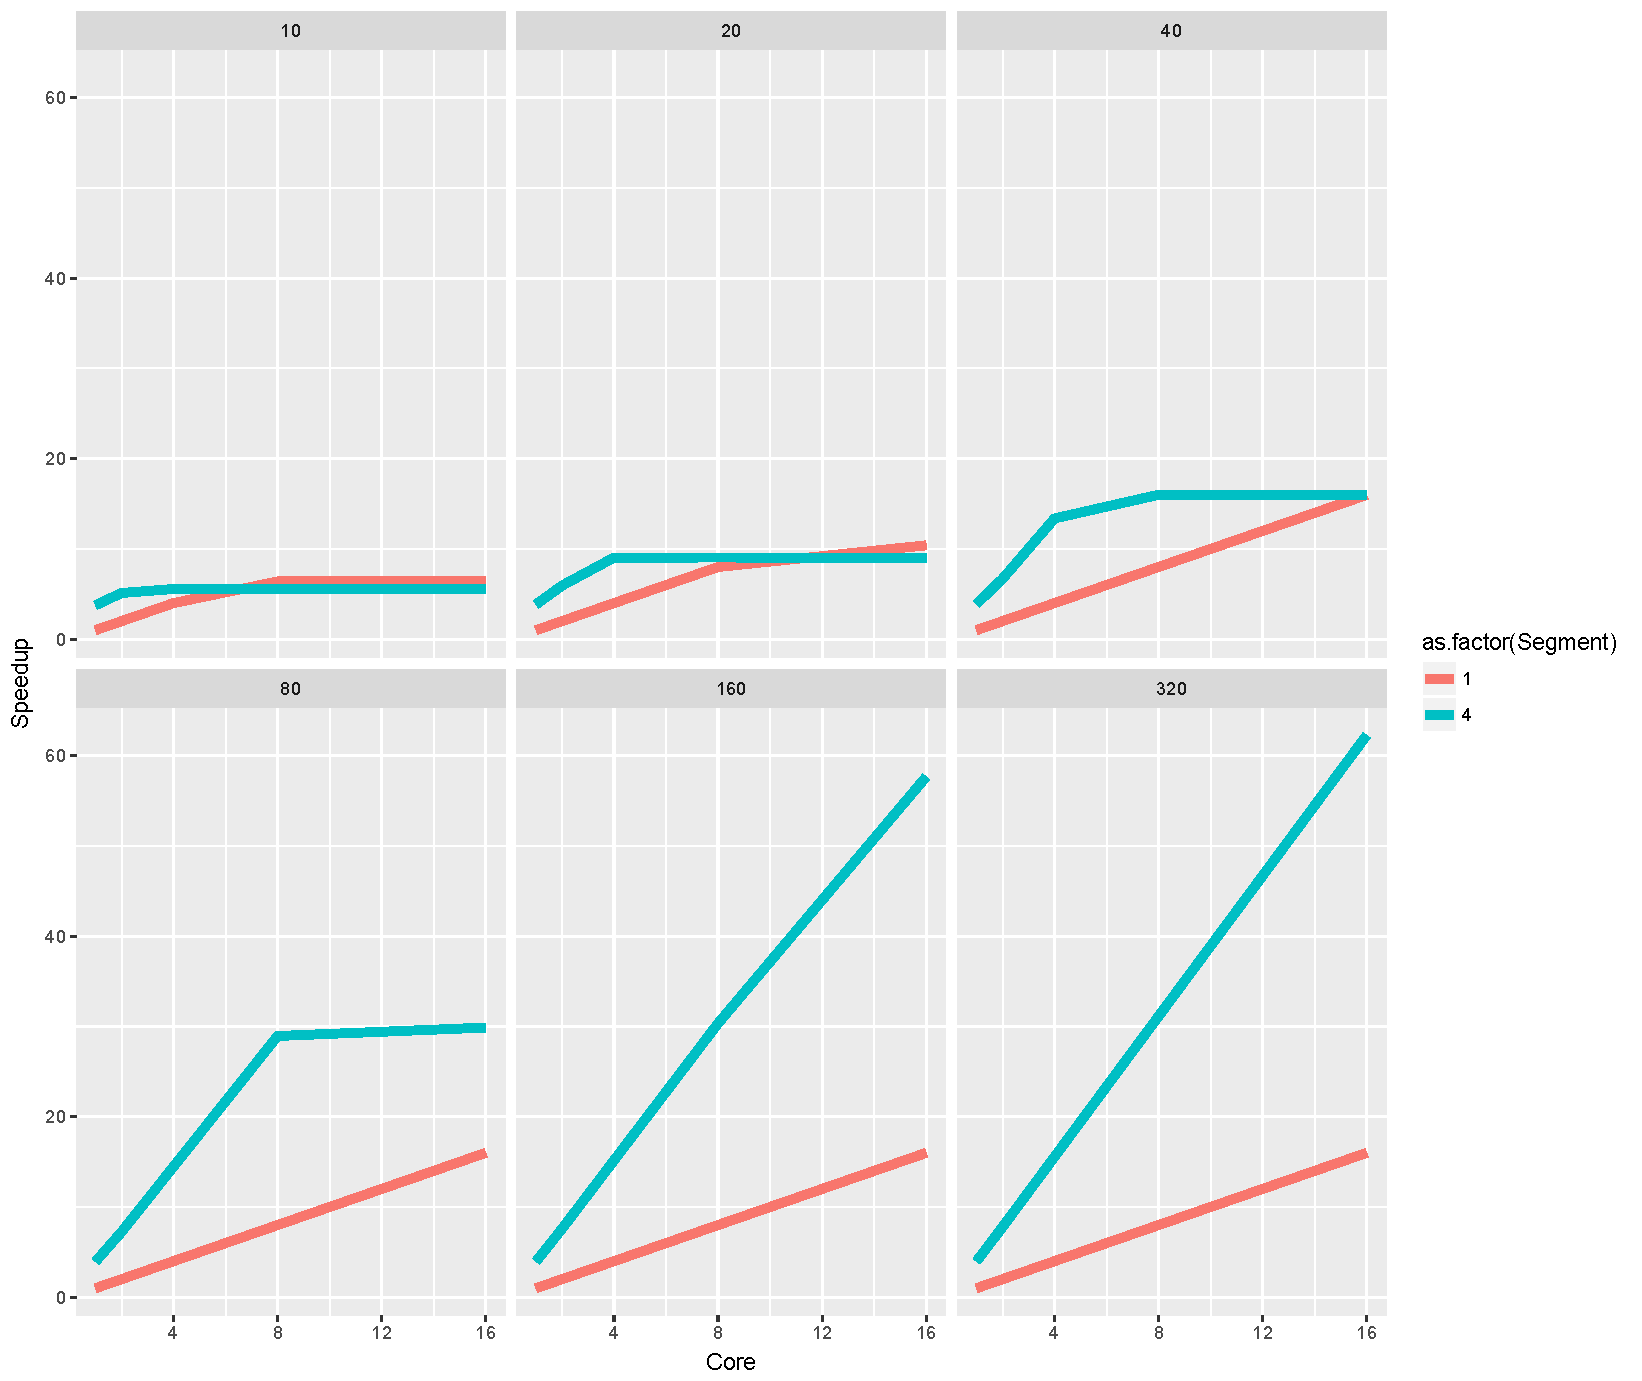
\includegraphics[width=1\textwidth]{chapter3/graphics/total_speed.pdf}
  \caption{Maximum speedup compared to 1 Core 1 Segment}\label{fig:ts}
\end{figure}

\subsection{Comparing segment performanced based on block size (in bytes)}

When blocks are larger than a single icache line, they must be fetched in multime cycles (according to the simulator implementation).
Naturally, we are not always likely to find blocks that fit in a single cache line, even when they are under 25 instructions.
For example we can have floating point instructions with immediates that take up the full 64 bits.
In this section, we look at how changing the size of a 25 or less instructions block will affect performance based on the segments. 
To run experiments, I created blocks of different sizes by injecting floating point operations that use immediates.
This ensures that the blocks can be large whilst staying 25 instructions or less.

Figure~\ref{fig:svl} shows the results of changing the size (in bytes) of a block, given a number of cores fused, the execution time in cycles of a block and the number of segments.
The speedups are obtained in the same fashion as in Figure~\ref{fig:lss}, that is to say I compared 1 Core 1 Segment with 16 Cores 1 Segment or 1 Core 4 Segments with 4 Core 4 Segments (I pair by segment).
In Figure~\ref{fig:svl} the X-Axis facet represents the block size, in this case either 16,40,84,172 or 228 bytes, given that an Icache line in this scenario is 32 bytes.
The Y-axis facet represents the execution time in cycles of a single block, just like in the previous examples.

As we can see from Figure~\ref{fig:svl}, the size of a block does not affect the speedup of single segment cores.
This is to be expected as a fetch request can be sent to another core before the fetch completion of a current block.
Therefore on a single segment, the number of i-cache line requests will not affect the actual performance scaling of adding more cores to a composition.
On the other hand this is clearly not the case for multi-segment cores.
This is simply due to the current limitations of the implementation of the fetching system in the simulator.
Since a core cannot fetch more than a single block at a time for itself, it will have to wait for the current block to finish before fetching the next block.
This does not stop it from sending a fetch request, but it means that it wont act upon that request before the current block is fully fetched.
Because of this, having larger blocks (in bytes) will increase the fetch length drastically.

Now, if the simulator implementation is not the correct implementation (and thus has been incorrect since forever), this would not necessarily fix every problem.
Instead, we would simply end up with the results from Figure~\ref{fig:lss} where we require blocks with long execution time to fully utilise the cores.
This is due to the fact that predictions are still serialised and also happen in a Core-order fashion.
\subsection{Branch Prediction}
In the CASES paper I make the claim that, for a core composition of \textit{X} number of cores, with \text{Y} number of segments must predict $(X*Y)-1$ blocks to ensure every core is fully utilised.
This is due to the fact that there is always a non-speculative block being executed in the chain, so this requires 1 less block to be predicted.
Naturally, this is to ensure full utilisation of every core; in a 4 segmented core, if we are able to correctly predict the first block of the 16th core, then we know that it will at least be used correctly to a certain extent.
Following the equation, I make the claim that we require a certain branch prediction rate to ensure the full utilisation of a core composition.
This equation is simply the number of blocks predicted over the total number of blocks in flight.
For example if we have a 16 core composition with 4 segmented cores, that's 63 divided by 64 so 98\%.
The phrasing I chose in the paper is actually somewhat awkward, as this percentage is a very precise number.
Instead of it being the branch prediction accuracy over the entire application it's actually the branch prediction for a specific \textit{string} of predictions.
Indeed, with a 98\% branch prediction accuracy, if the 1 mispredicted block is the second block in the chain, then the rest of the fetched blocks will still be useless.
So only specifying a percentage is not an accurate representation of what I was trying to convey.
I therefore need to reformulate this percentage of branch prediction accuracy to better describe the problem at hand (and errata it from the previous paper).

\subsection{Conclusion}

Overall we have seen how sensitive 4 segment cores can be; currently they require longer blocks but also require these blocks to not have such a heavy size footprint.
Whilst this may be the case, 4 segments can help alleviate the work from the compiler side as we can fit more blocks onto a single core.
They also provide flexibility, as when blocks grow in terms of instruction size, they become more and more like single-segmented cores.
Since we know that large blocks often require some form of hyper-block formation, which, without profiling information may lead to blocks that contain a lot of wasted space, having the opportunity to fetch more blocks should be much more beneficial.
More segments should also provide more interesting opportunities for scheduling blocks as they allow for more blocks in flight.

\begin{figure}
\center
  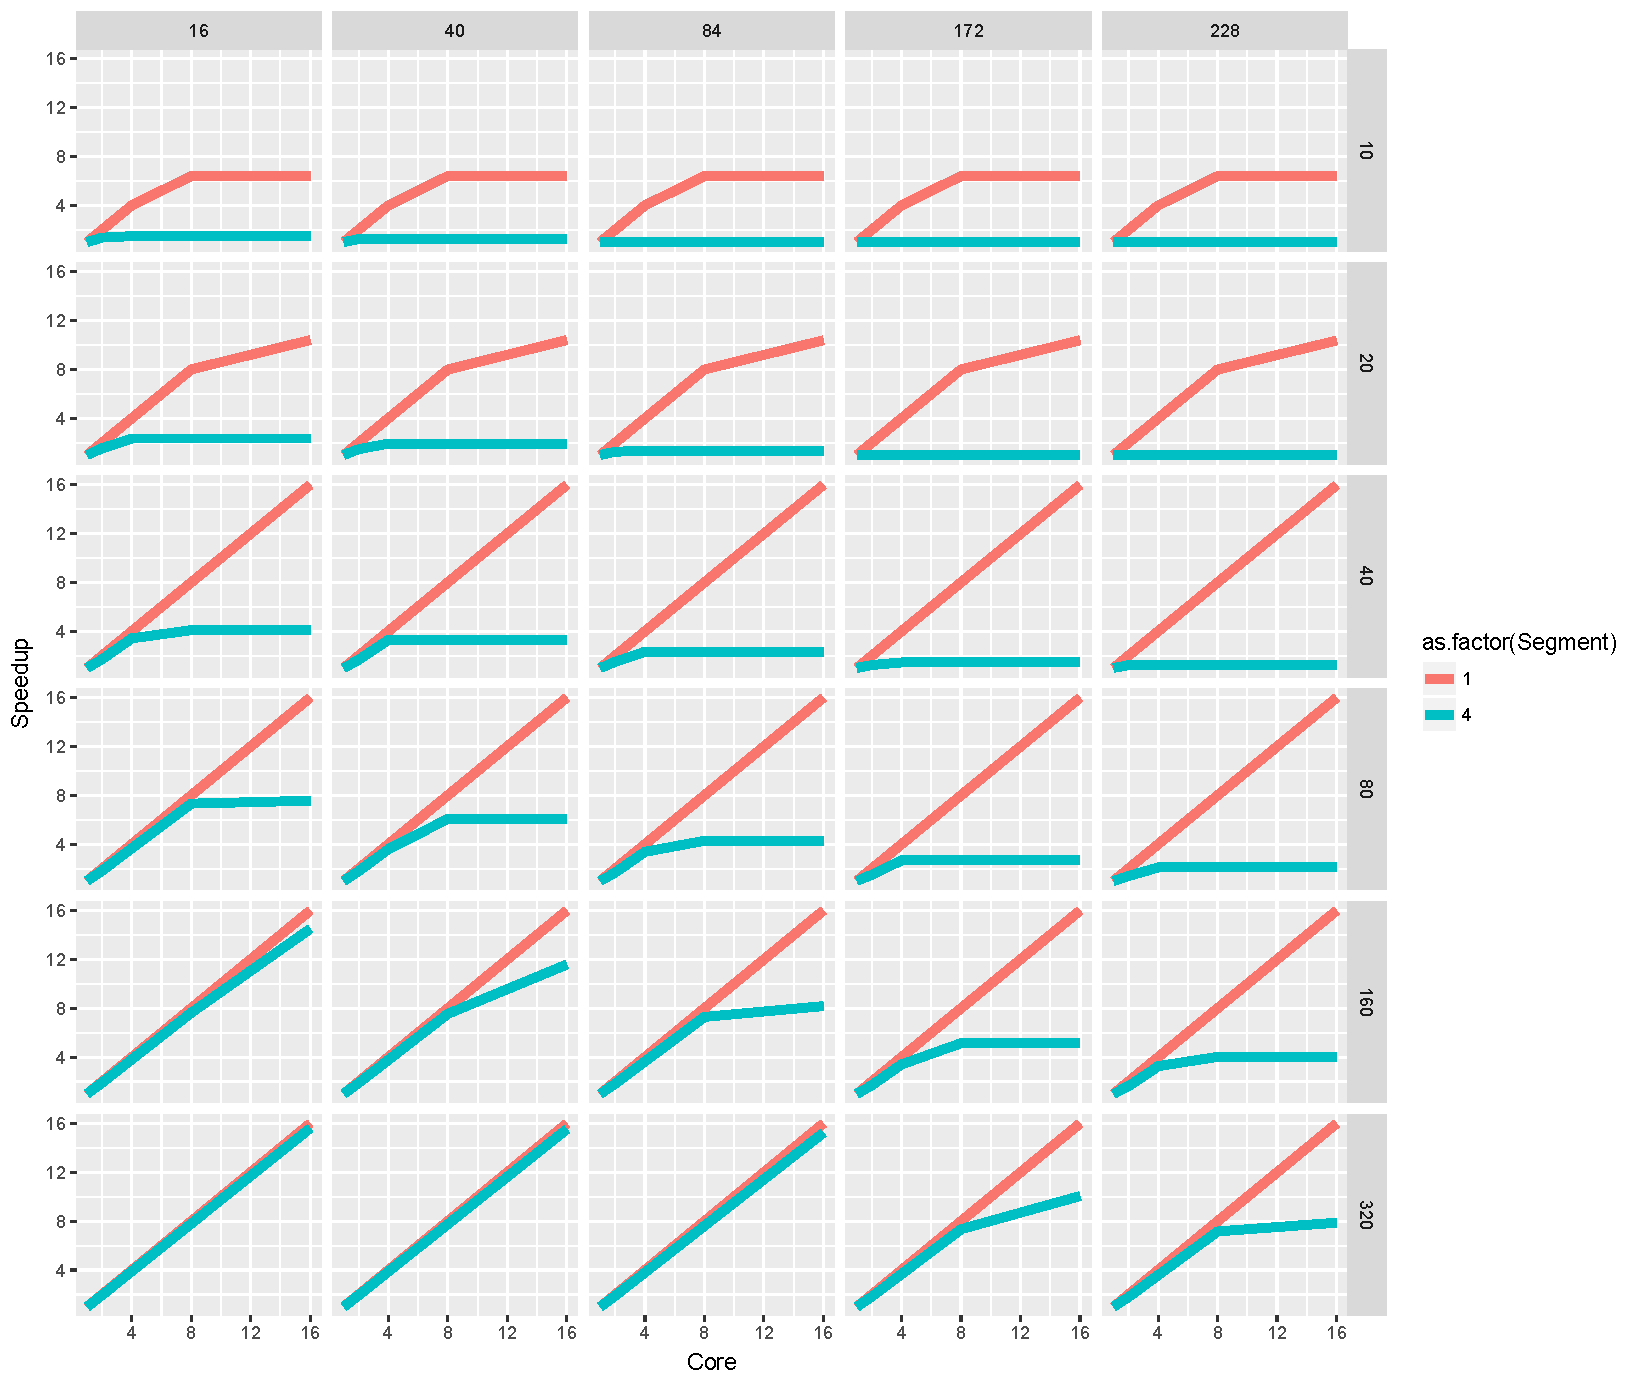
\includegraphics[width=1\textwidth]{chapter3/graphics/size_vs_length.pdf}
  \caption{Speedup by segments.}\label{fig:svl}
\end{figure}

\newpage
\section{What can we do about it?}

\subsection{Unlocking block dispatch}

Currently a core cannot issue a new block if its youngest segment has already submitted a fetch request.
This current restriction means that blocks have to be submitted to cores in a sequential fashion, in other words, if we have 2 cores in a fusion, then C1 cannot fetch a block, send another block to C2 and then fetch a 3rd block. Instead, once it has submitted a block to C2 it will \textbf{have} to wait for C2 to send a new block.
This is what is currently causing cores to wait. Once they have submitted a block to another core, even if their youngest segment commits, they must wait for all other cores in the composition to have fetched blocks so that the fetching wraps back to it.

What I propose as a first step is to try and explore new fetching mechanisms for core-fusion, mainly pipelining fetches.
Instead of "fetching until you're full", a core should start off by making 1 prediction for itself and 1 prediction for the next core in the fusion.
Once it has executed this step it can continue fetching 3 other blocks whilst the next core repeats the process.
This should ensure all cores are fetching 4 blocks almost in parallel.
A paper from 1996 by Andre Seznec et al. from INRIA proposed a multi-block branch predictor that can generate 2 predictions in a single cycle.
We could use this work to do predictions for number of blocks.

Currently, if we have 16 cores, each fetching 4 blocks, if we assume that it takes at least 4 cycles to fetch a block and send a prediction, we have
$fetchlat=(16 * 4)*4$  so 256 cycles before each core has filled up.
By pipelining we can reduce this down to $fetchlat=4+(15*4)+4$  so 68 cycles which is a 3.7x speedup.
Refering back to Figure~\ref{fig:lss}, having an overhed of 68 cycles would place us between the 40 and 80 cycles facet, which means that if we are able to maximize speedup around those facets, that's a 2.6x speedup for a 16 core, 4 segment fusion.
This should, in theory, allow us to better utilise core-fusion as it decreases the restrictions on how long a block should take to execute for a given core-composition size.
Let's recall in the previous report that the overall speedup of a loop, when we only have a single segment can be measured by:
\begin{equation}\label{eq:avspeed}
\frac{Average Execution Time}{\frac{4+4*(Cores -1)+ Average Execution Time + Dependencies  * Cores}{ Cores}}
\end{equation}

In this formula, $4+4*(Cores-1)$ represents the fetch overhead when we have a single segment.
Currently, on 4 segments this would be $4+4*(Cores-1)*4$ which reduces the potential speedup window.

\subsection{Improving branch prediction requirements}

We can use this oportunity of exploring how blocks are fetched to improve overall core-utilisation by ordering the blocks in a different manner.
As we state in the CASES paper, for a core to be useful in a core-fusion, all previous blocks must have been accurately predicted, which can be a huge strain on the branch predictor.
If, instead, we were to send the first prediction made by a core to the following core, we can reduce the stress on the branch predictor.
For example if we had 4 Cores, C1 would have blocks [1,5,9,13] C2:[2,6,10,14], C3:[3,7,11,15] and C4:[4,8,12,16].
In this case, we only need to make 3 predictions to ensure that C4 has at least been somewhat useful.
Previously, in a 16 core composition, if we had 64 blocks in flight, the 16th core could only be considered useful if 60 out of the 64 blocks were considered correct.
This implied at least a 93.7\% accuracy just to ensure that all cores were running some correct code whereas in this new model, only 15 predictions would ensure a utilisation of the core, so dropping it to a mere 23\%.
In Core-Fusion by Ipek et al. Figure 9 shows the distribution of fetch cycles for SPECINT and SPECFP benchmarks.
They define 4 categories: pipeline stalls (cores are busy executing), wrong path (misprediction), FMU stalls (stalls caused by communicating to FMU) and true fetch, which I assume is cycles spent doing actual fetch work.
Whilst they claim that the FMU only causes a 3\% overhead in fetch cycles, they fail to address the fact that, for some benchmarks in SPECINT, mispeculation can caust them up to 50\% of their fetch cycles which is huge.
In these cases they percieve no speedup since they're getting branches wrong almost half the time.
By changing the scheme we can claim that we maintain a higher number of live blocks whilst allowing cores to be useful more frequently.

\subsection{Exploring smarter schedulers}

A lot of the talk in this report is somewhat focused on trying to tackle fetching overhead when we assume blocks are small and take no time to execute.
This most often will only occur in integer heavy blocks, or situations where all data is in cache and blocks are small due to heavy control flow.
However this isn't always the case, and blocks can take a long time to execute.
In these situations, the overhead of fetching isn't the problem but rather which blocks are being fetched and dispatched.
Since we're playing around with how blocks are dispatched we may use this oportunity to look at loops 

\subsection{Introduce a new architecture module}

My plan is to introduce a small module to the architecture which can handle fetch requests made by different cores.
Instead of having a round-robin model, where cores only make fetch requests to other cores once they're full, I intend on having cores submit fetch requests to a module which every core can ping when they are empty.
Using a branch predictor that can make 2 predictions per cycle, we can have each core fetch a block for themselves and send another one to this new module.

The module would simply be a queue that contains a block address and, maybe, the size of the block (in instructions).
The size of the block could be taken from some very small cache, since we don't expect to ever have hundreds of fetch requests being made.
Having the block size in instructions will help avoid situations in which cores pop a request from the module but can't service it due to insufficient segments.
The size should be counted in segments rather than instructions as this reduces the space to a 3 bit field.
I also think we could extend this module to contain a field for scheduling blocks on specific cores.
This way if we, for example, want to schedule blocks in a specific order, we can use this module to filter blocks.
If we can have up to 16 cores in a composition, then that leads to a 4 bit field identifier.
So overall we would only need to cache 7 bits, + some tag to make sure we're pulling the right information (since we can use the address as way to find a cacheline).

\section{How we should evaluate}

\subsection{Simulator}

There are some modifications that have been made and will need to be made to get the results we need.
As of now I have these things implemented:

\begin{itemize}
\item Define custom cycle counts for specific instructions
\item Define a custom branch-prediction accuracy
\item An ITTAGE branch predictor that can be customised to potentially generate 2 predictions per cycle
\item A high-level L2 cache simulation (not very accurate as far as banks or signals go)
\end{itemize}

\subsection{Synthetic Benchmarks}

The first and quickest method of evaluating how block fetching can impact performance is through synthetic benchmarks.
As of now I can think of 3 important parameters for synthetic benchmarks: block size (bytes), block length (cycle), and branch prediction.
By changing these parameters we can determine the most "resilient" method.
Ultimately we want to demonstrate that the current method is ineffective for a large variety of blocks, and also has very little resistance to sequential branch misprediction.

\subsection{Actual benchmarks}

I want to focus on single threaded benchmarks that can help us demonstrate how new block-fetching and block-scheduling algorithms can outperform a more traditional straight forward serial implementation that we have currently.
We essentially want to focus on loops that have a combination of these features:
\begin{itemize}
\item A lot of if-statements (to stress-test branch prediction)
\item Data dependencies
\item Independent iterations
\end{itemize}
I can't think of many more things right now but these can easily come later.